\documentclass{standalone}
\usepackage{tikz}
\usepackage{mathrsfs}
\usetikzlibrary{positioning, shapes.geometric, arrows}
\tikzstyle{startstop} = [draw, rectangle, rounded corners, minimum width=3cm, minimum height=1cm,text centered, draw=black]
\tikzstyle{bola} = [draw, circle , minimum size = 10, draw=black, text centered]
\tikzstyle{elipse} = [draw, ellipse, minimum height = 10]
\usepackage[T1]{fontenc}
\renewcommand*\familydefault{\ttdefault} %% Only if the base font of the document is to be typewriter style
\begin{document}
\begin{tikzpicture}
	
	\draw (0,0) rectangle (6,0.5);
	\draw [<->] (0,-2) -- (6,-2);
	\draw (0,-1.9) -- (0,-2.1);
	\draw (6,-1.9) -- (6,-2.1);
	\draw [color=red] (5,-1.7) node {$1$};
	
	\only<1>{\draw (6, 1.5) node {Tomamos el valor de $1$};}
	
	\pause

	
	\draw (0,-0.1) rectangle (3,-0.6);
	\draw [dashed] (3,-0.6) -- (3, -2.4);
	\draw [<->] (0,-2.4) -- (3,-2.4);
	\draw [color=red] (2.7,-1.7) node {$\frac{1}{2}$};
	
	
	\only<2>{\draw (6, 1.5) node {Dividimos a la mitad esta unidad};}

	\pause
	
	\draw (0,-0.7) rectangle (1.5,-1.2);
	\draw [dashed] (1.5,-1.2) -- (1.5, -2.6);
	\draw [<->] (0,-2.6) -- (1.5,-2.6);
	\draw [color=red] (1.3,-1.7) node {$\frac{1}{4}$};
	
	\only<3>{\draw (6, 1.5) node {Volvemos a dividir a la mitad};}


	\pause

	\draw (0,-1.3) rectangle (0.75,-1.8);
	\draw [dashed] (0.75,-1.8) -- (0.75, -2.9);	
	\draw [<->] (0,-2.9) -- (0.75,-2.9);
	\draw [color=red] (0.7,-3.3) node {$\frac{1}{8}$};

	\draw (6, 1.5) node {Seguimos dividiendo a la mitad ...};
\end{tikzpicture}
\end{document}